\documentclass[12pt, letterpaper]{article}
\usepackage[titletoc,title]{appendix}
\usepackage{color}
\usepackage{booktabs}
\usepackage{dcolumn}
\usepackage[usenames,dvipsnames,svgnames,table]{xcolor}
\definecolor{dark-red}{rgb}{0.75,0.10,0.10}
\definecolor{bluish}{rgb}{0.05,0.05,0.85}

\usepackage[margin=1in]{geometry}
\usepackage[linkcolor=blue,
			colorlinks=true,
			urlcolor=blue,
			pdfstartview={XYZ null null 1.00},
			pdfpagemode=UseNone,
			citecolor={bluish},
			pdftitle={exp_partisan_gap}]{hyperref}

\usepackage[resetlabels,labeled]{multibib}
\newcites{SI}{SI References}
\usepackage{natbib}

\usepackage{float}

\usepackage{geometry} % see geometry.pdf on how to lay out the page. There's lots.
\geometry{letterpaper}               % This is 8.5x11 paper. Options are a4paper or a5paper or other... 
\usepackage{graphicx}                % Handles inclusion of major graphics formats and allows use of 
\usepackage{verbatim}
\setcitestyle{round,semicolon,aysep={},yysep={;}}
\usepackage{setspace}		     % Permits line spacing control. Options are \doublespacing, \onehalfspace
\usepackage{sectsty}		     % Permits control of section header styles
\usepackage{pdflscape}
\usepackage{fancyhdr}		     % Permits header customization. See header section below.
\usepackage{url}                     % Correctly formats URLs with the \url{} tag
\usepackage{fullpage}		%1-inch margins
\usepackage{multirow}
\usepackage{rotating}
\setlength{\parindent}{3em}

\usepackage[T1]{fontenc}
\usepackage[bitstream-charter]{mathdesign}

\usepackage{chngcntr}
\usepackage{booktabs}
\usepackage{longtable}

\def\citeapos#1{\citeauthor{#1}'s (\citeyear{#1})}

\makeatother

\usepackage{footmisc}
\setlength{\footnotesep}{\baselineskip}
\makeatother
\renewcommand{\footnotelayout}{\normalsize \doublespacing}


% Caption
\usepackage[hang, font=small,skip=0pt, labelfont={bf}]{caption}
%\captionsetup[subtable]{font=small,skip=0pt}
\usepackage{subcaption}

% tt font issues
% \renewcommand*{\ttdefault}{qcr}
\renewcommand{\ttdefault}{pcr}

\setcounter{page}{0}

\usepackage{lscape}
\renewcommand{\textfraction}{0}
\renewcommand{\topfraction}{0.95}
\renewcommand{\bottomfraction}{0.95}
\renewcommand{\floatpagefraction}{0.40}
\setcounter{totalnumber}{5}
\makeatletter
\providecommand\phantomcaption{\caption@refstepcounter\@captype}
\makeatother


\title{An Unclear Gap: How Vague Response Options Produce Partisan Knowledge Gaps \thanks{Replication materials posted at: \url{ https://github.com/soodoku/unclear_gap}}}

\author{Carolyn E. Roush\thanks{\href{mailto:carolyn.roush@gmail.com}{\texttt{carolyn.roush@gmail.com }}} \and Gaurav Sood\thanks{\href{mailto:gsood07@gmail.com}{\texttt{gsood07@gmail.com}}}}

\begin{comment}

setwd("~/Documents/Github/unclear_gap/ms/")
tools::texi2dvi("unclear_gap.tex", pdf = TRUE, clean = TRUE)

\end{comment}

\begin{document}
\maketitle
\thispagestyle{empty}

\begin{abstract}

\noindent \citet{roush_2021} use a dataset of 162,083 responses to 187 items on 47 surveys to find that partisan gaps are smaller and less frequent than commonly understood. The average is a mere six and a half points and gaps' ``signs'' run counter to expectations roughly 30\% of the time. However, one exception is the size of gaps on retrospection items on the ANES, which are considerably bigger. These retrospection items use vague response options, e.g., `About the same.' Vague response options can inflate partisan gaps by offering partisans the opportunity to interpret the same data differently. We test this assumption with a novel survey experiment. We present partisans data indicating a small improvement in economic indicators and manipulate the partisan tint of the change by manipulating who is responsible for the change. We find that significantly fewer partisans pick the option that '[things] got better' when presented with an out-partisan cue than a co-partisan cue. Our findings suggest that vague options can induce knowledge gaps where none exist.
\end{abstract}

\vspace{.2in}


\newpage

\doublespacing
Data from \citet{roush_2021} suggest that partisan knowledge gaps are highly variable and that large differences in what Democrats and Republicans believe are less common than what many assume. If partisan gaps are small on average, why does the common wisdom that Democrats and Republicans differ substantially in political knowledge persist? 

One explanation for this discrepancy is that conventional wisdom is largely based on studies using data from the \citet{anes_gen}. But there may be a good reason to think that the gaps in the ANES data are not representative of broader trends in partisan knowledge differences. Unlike most knowledge questions---which require partisans to identify an objectively correct answer---most ANES questions about party consequential ``factual beliefs'' do not ask respondents to do the same. Instead, these questions ask respondents to make subjective \textit{assessments} about performance or policy over a certain time period. Canonical ANES questions, for example, ask people to gauge whether the budget deficit increased, decreased, or remained about the same over a president's tenure, or how the rate of inflation changed over the past year. Because the response options for these questions---``got better,'' ``stayed about the same,'' or ``got worse''---are imprecise, people have a greater opportunity to interpret the meaning themselves \citep[e.g.][]{beyth_1982} using common heuristics, including partisanship \citep[e.g.][]{soodguess_2017}. As a result, a large partisan ``knowledge'' gap may reflect how partisans interpret response options rather than a true difference between what Democrats and Republicans know.

This is particularly problematic for cases where changes in inflation, unemployment, the deficit, or other performance items are marginal. While there are certain contexts---such as a stock market crash---where unambiguous evidence forces partisans to acknowledge the same economic reality \citep[e.g.][]{bisgaard2015bias,parkerstephen_2013}, far more survey questions are asked in times when performance indicators change gradually over time. When researchers ask respondents to classify these changes in performance indicators using vague response options, it opens the door for partisan bias even if individuals know the same objective information. Consider the case of two highly knowledgeable survey respondents (who perhaps work in the Bureau of Labor Statistics) who know definitively that the national unemployment rate in the United States grew from 4.0\% to 4.2\% over the past year, a time during which a Republican president occupied the White House. When the first respondent, a Democrat, is asked to evaluate how unemployment changed over the past year, she might (correctly) reason that unemployment ``got worse'' as the rate objectively increased over the previous 12 months. On the other hand, the second survey respondent, a Republican, might also (reasonably) conclude that 0.2 percentage points is a negligible change in unemployment, and might therefore be more liable to answer that the unemployment rate  ``stayed about the same'' over the past year. In this situation, two people who know \textit{the exact same fact} could plausibly choose two different response options and still be correct. The end result is that some ``knowledge gaps'' may be artificially large simply because respondents interpret the same response categories differently. 

To test this hypothesis, we first examined the average size of partisan knowledge gaps that occur in ANES data and compared them to the average partisan gaps in other studies. To do so, we relied on the data compiled by \citet{roush_2021}: all knowledge items that carry a partisan implication that appeared on ANES surveys over the past 32 years.

Table 1 compares partisan gaps on ANES items to those included in the other studies in our analysis. As expected, the mean and median gaps on ANES knowledge items are substantially larger than those in the other three studies. In fact, the mean partisan knowledge gap in the ANES data (17 percentage points) is more than 50\% larger than the largest average gap in any other study (10 percentage points, from \citet{bullocketal_2015}). Furthermore, only two of the 28 items taken from ANES surveys produce negatively-signed partisan gaps, and only five of these items produce knowledge gaps that are not statistically significant at the 95\% confidence level. While the sample size of questions taken from the ANES is small, it is clear that the partisan gaps produced from these items are markedly larger.

% latex table generated in R 4.1.2 by xtable 1.8-4 package
% Sat Jan 01 22:31:42 2022
\begin{table}[!htb]
\centering
\begin{tabular}{lrrrr}
  \hline
Study & Mean Gap & Median Gap & SD & N(Items) \\ 
  \hline
ANES & 0.168 & 0.139 & 0.139 &   28 \\ 
  Bullock et al. & 0.104 & 0.089 & 0.119 &   21 \\ 
  Jerit \& Barabas & 0.036 & 0.032 & 0.091 &  128 \\ 
  Prior et al. & 0.063 & 0.035 & 0.093 &   10 \\ 
   \hline
\end{tabular}
\caption{Partisan Gap by Study} 
\label{tab:tab_1}
\end{table}


Our hunch is that these large gaps are a result of vague response categories that allow partisans to classify the same information in different ways. To test this hypothesis, we conducted an original experiment using Amazon's Mechanical Turk (MTurk) in June 2020. In the study, we provided all respondents with a question prompt that featured real economic information about the change in the inflation and unemployment rates during 2016.\footnote{This information was collected from the U.S. Bureau of Labor, available at \begin{footnotesize} \url{https://data.bls.gov/timeseries/lns14000000}.\end{footnotesize}} In addition to providing this information, we randomly assigned respondents to one of two treatments: one that attributed these changes to then-Democratic President Barack Obama and the other that attributed the changes to the Republican-controlled Congress. We then asked respondents to classify these changes using the canonical ANES response categories (``got worse,'' ``stayed about the same,'' or ``got better''). The specific treatment was as follows: 

\begin{quotation} 
\noindent \textit{During 2016, (when Barack Obama was president | when Republicans were in control of both Houses of Congress), unemployment decreased from 5.0\% to 4.8\%, a change of 0.2 percentage points. How would you interpret this change? Would you say that unemployment got better, stayed about the same, or got worse?}

\bigskip

\noindent \textit{In 2016, inflation also decreased from 2.1\% to 1.9\%, a change of 0.2 percentage points. How would you interpret this change? Would you say that inflation got better, stayed about the same, or got worse?}

\end{quotation}

Since prior research demonstrates that partisans evaluate economic conditions favorably when their own party is in power and unfavorably when the other party is in power \citep[e.g.][]{bartels_2002,bisgaard2015bias}, we expected respondents to classify objective economic information differently depending on the partisan cue they received. Specifically, we expected that partisans would be more likely to classify a 0.2 reduction in the unemployment or inflation rates as having ``got[ten] better'' under co-party leadership and as having ``stayed about the same'' (or ``got[ten] worse'') under the opposing party's leadership. For ease of interpretation, we recoded the data so that treatments and respondents are characterized in relation to one another: we classified Democrats who saw the President Obama cue and Republicans who saw the Republicans-in-Congress cue as receiving an \textit{In-party cue} and Democrats who saw the Republicans-in-Congress cue and Republicans who saw the President Obama cue as having received an \textit{Out-party cue}).\footnote{Consistent with previous research \citep[e.g.,][]{keithetal_1992}, we classify Independent leaners as partisans.} 

Figure \ref{fig:combined_exp} presents the distribution of responses by experimental conditions for both dependent variables. As we can see, partisans classify a small, 0.2 percentage point change in unemployment or inflation very differently depending on the party to which the change was attributed. Respondents who received the \textit{Out-party cue} were, on average, 21.5 percentage points less likely than those receiving the \textit{In-party cue} to view the reduction in the unemployment rate as having ``got[ten] better'' during 2016. Respondents who received the \textit{Out-party cue} were about 18 percentage points less likely than \textit{In-party cue} respondents to classify the reduction in unemployment as ``stayed about the same.'' We find similar results for inflation, albeit with somewhat smaller effects: those who received the \textit{Out-party cue} were approximately 16 percentage points less likely than those who received the \textit{In-party cue} to classify the 0.2 reduction in inflation as having ``got[ten] better;'' those who received the \textit{Out-party cue} were also 13.6 percentage points more likely than \textit{In-party cue}-receivers to classify the change as ``stayed about the same.''


\begin{center}
\begin{figure}[H]
  \centering
  \caption{\textit{Distribution of Dependent Variables by Experimental Condition}}
  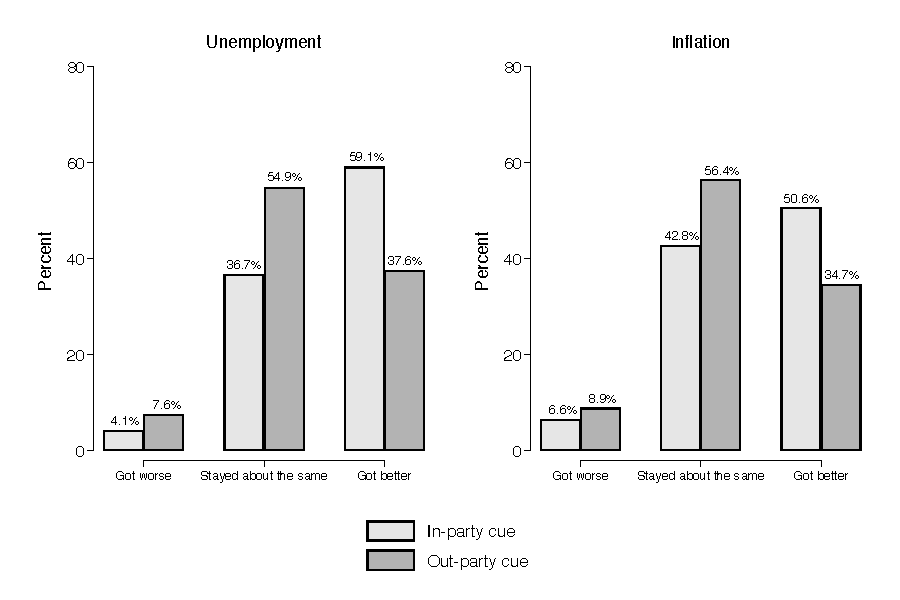
\includegraphics[width=\textwidth]{../figs/combined_nontroll.pdf}
  \label{fig:combined_exp}
\end{figure}
\end{center}

\vspace{-2.5cm}

We also estimated two regression models predicting evaluations of unemployment and inflation (where 1 = ``got better,'' 0.5 = ``stayed about the same,'' and 0 = ``got worse'') as a function of whether or not respondents received the \textit{Out-party cue}. The results of this analysis can be found in Table \ref{tab:tab_3}.\footnote{In recent years, researchers have noted that significant portions of the data collected on MTurk is of questionable quality, provided either by respondents who provide misleading information regarding the location from which they are completing a \texttt{HIT} or who provide humorous or insincere responses to survey questions \citep[e.g.,][]{turk_paper,mturk_2019,bai_2018,dreyfuss_2018,kennedy2019shape,ryan_2018}. As demonstrated by  \citet{turk_paper} and \citet{kennedy2019shape}, these bad actors can attenuate treatment effects by introducing noise into the data. Accordingly, we followed the recommendations of \citet{turk_paper} and \citet{kennedy2019shape} to identify these suspicious responses and only present results among non-suspicious respondents in both Figure \ref{fig:combined_exp} and Table \ref{tab:tab_3} (\textit{n}=861). Consistent with previous research, we find that suspicious respondents attenuated treatment effects. Nevertheless, we still find impressive effects when including suspicious respondents in our analysis: among the full sample (\textit{n}=1,425), receiving the \textit{Out-party cue} causes respondents to view the change in unemployment 9.6 percentage points more negatively and the change in inflation 6.0 percentage points more negatively than those respondents who received the \textit{In-party cue}. For more information, please see \ref{si:exp_results_full}.} Consistent with the results in Figure \ref{fig:combined_exp}, partisans who received the \textit{Out-party cue} were less likely than respondents who received the \textit{In-party cue} to view (normatively positive) reductions in unemployment and inflation favorably. Specifically, those respondents who were told that an out-party leader oversaw the reduction in the unemployment rate viewed the change 12.5 percentage points less favorably than those who received the \textit{In-party cue}. Similarly, respondents who received the \textit{Out-party cue} viewed the reduction in the inflation rate 9.1 percentage points less favorably than those who received the \textit{In-party cue}. The magnitude of these effects is sizeable.

\begin{table}[h]
\caption{\textit{Impact of Treatment on Economic Evaluations}\label{tab:tab_3}}
\begin{center}
\begin{tabular}{lcc} \hline
 & Unemployment & Inflation \\ \hline
 &  &  \\
Out-party cue & -0.125*** & -0.091*** \\
 & (0.020) & (0.021) \\
Constant & 0.775*** & 0.720*** \\
 & (0.015) & (0.015) \\
 &  &  \\
Observations & 861 & 861 \\
 R-squared & 0.043 & 0.022 \\ \hline
  & & \\
\multicolumn{3}{c}{\begin{footnotesize} Standard errors in parentheses. \end{footnotesize}} \\
\multicolumn{3}{c}{\begin{footnotesize} ***\textit{p}$<$0.01, **\textit{p}$<$0.05, *\textit{p}$<$0.1, two-tailed. \end{footnotesize}} \\
\multicolumn{3}{c}{\begin{footnotesize} All variables have been rescaled 0-1 for ease of interpretation.\end{footnotesize}} \\
\end{tabular}
\end{center}
\end{table}


We replicated the experiment on Lucid in 2023. Table ~\ref{lucid} presents the results. Once again, we see that respondents are less likely to pick the option that things are getting better when we present an uncongenial cue versus a scenario where we present a congenial cue. 


\begin{table}[!htbp] \centering 
  \caption{Impact of Treatment on Economic Evaluations (Lucid)} 
  \label{lucid} 
\begin{tabular}{@{\extracolsep{5pt}}lD{.}{.}{-3} D{.}{.}{-3} } 
\\[-1.8ex]\hline 
\hline \\[-1.8ex] 
 & \multicolumn{2}{c}{\textit{Dependent variable:}} \\ 
\cline{2-3} 
\\[-1.8ex] & \multicolumn{1}{c}{Unemployment} & \multicolumn{1}{c}{Inflation} \\ 
\\[-1.8ex] & \multicolumn{1}{c}{(1)} & \multicolumn{1}{c}{(2)}\\ 
\hline \\[-1.8ex] 
 Out-party cue & -0.072^{**} & -0.102^{***} \\ 
  & (0.030) & (0.030) \\ 
  & & \\ 
 Constant & 0.741^{***} & 0.771^{***} \\ 
  & (0.021) & (0.021) \\ 
  & & \\ 
\hline \\[-1.8ex] 
Observations & \multicolumn{1}{c}{529} & \multicolumn{1}{c}{529} \\ 
R$^{2}$ & \multicolumn{1}{c}{0.011} & \multicolumn{1}{c}{0.021} \\ 
\hline 
\hline \\[-1.8ex] 
\textit{Note:}  & \multicolumn{2}{l}{$^{*}$p$<$0.1; $^{**}$p$<$0.05; $^{***}$p$<$0.01} \\ 
 & \multicolumn{2}{l}{Standard errors in parentheses.} \\ 
 & \multicolumn{2}{l}{All variables have been rescaled 0-1 for ease of interpretation.} \\ 
\end{tabular} 
\end{table} 


Our results suggest that a significant portion of partisans' disagreement about the ``acceptance of basic political facts, such as the state of the economy'' \citep[211]{berinsky_2017} might be better explained as a biased interpretation of response categories rather than genuine differences in knowledge. Even when partisans are presented with the \textit{exact same} factual information, they classify it differently based upon their preexisting biases and political context (see also \citeauthor{gainesetal_2007} \citeyear{gainesetal_2007}). The fact that vague response options are common on the ANES---perhaps the most commonly used source of public opinion data in the discipline---helps contribute to the (mistaken) belief that differences in what Democrats and Republicans are large enough to warrant serious concerns about democratic accountability. 

\clearpage
\bibliographystyle{apsr}
\bibliography{pgap}

\clearpage

\appendix
\renewcommand{\thesection}{SI \arabic{section}}
\setcounter{table}{0}\renewcommand\thetable{\thesection.\arabic{table}}  
\setcounter{figure}{0}\renewcommand\thefigure{\thesection.\arabic{figure}}
\counterwithin{figure}{section}

\section{Question-Wording from June 2020 MTurk Experiment}
\label{si:exp_questions}

Switching gears, we'd like to understand how you think various measures of the economy performed a few years ago, \textit{(when Barack Obama was president | when Republicans were in control of both Houses of Congress).}

\bigskip

\noindent During 2016, \textit{(when Barack Obama was president | when Republicans were in control of both Houses of Congress)}, unemployment decreased from 5.0\% to 4.8\%, a change of 0.2 percentage points. How would you interpret this change? Would you say that unemployment got better, stayed about the same, or got worse? 

\begin{itemize}
\item Got better
\item Stayed about the same 
\item Got worse
\end{itemize}

\bigskip

\noindent In 2016, inflation also decreased from 2.1\% to 1.9\%, a change of 0.2 percentage points. How would you interpret this change? Would you say that inflation got better, stayed about the same, or got worse? 

\begin{itemize}
\item Got better
\item Stayed about the same 
\item Got worse
\end{itemize}

\clearpage


\section{MTurk Data Quality and Attenuation of Treatment Effects} \label{si:exp_results_full}

\begin{doublespace}

As mentioned previously, we followed the advice of \citet{turk_paper} and \citet{kennedy2019shape} to identify low-quality responses on Amazon's Mechanical Turk (MTurk). To do so, we first used a Qualtrics plugin to record the IP addresses from which respondents were taking the survey. We further collected IP-level metadata and flagged any respondent who took the survey from outside the United States (as the survey was limited to American adults), completed the survey more than once, or completed the survey from a blacklisted address as suspicious/of potential low-quality. In order to identify respondents who may provide humorous or insincere responses to survey questions, we also asked respondents a series of low-incidence screener questions. These questions ask about rare afflictions and behaviors, such as whether the respondent was a member of a gang, whether the respondent used a prosthetic, etc. Following \citet{turk_paper} and \citet{lopezhillygus_2018}, we classified any respondent as suspicious/a potential provider of low-quality data if they answered in the affirmative to two or more of these questions. In all, we found that 38\% of our data is of questionable quality. 

To determine whether low-quality responses attenuate treatment effects, we estimated four regression models in \ref{tab:treat_effects_complete}. For context, the first two models provide the results among the entire sample (including low-quality responses) using the unemployment and inflation dependent variables, respectively. The last two models include an indicator for whether the respondent was flagged as providing a \textit{Low-quality response} and an interaction term comprised of the \textit{Low-quality response} indicator and assignment to the \textit{Out-party cue} condition. As we can see, flagged respondents attenuate treatment effects for both dependent variables, but impressive effects remain: even when including low-quality respondents in our data, respondents are 9.6 percentage points less likely to view the change in unemployment as having ``gotten better'' and 6.0 percentage points less likely to view the change in inflation similarly under out-party leadership. 

\end{doublespace}

\begin{table}[H]
\caption{\textit{Impact of Low-Quality Responses on Treatment Effects}\label{tab:treat_effects_complete}}
\begin{center}
\begin{tabular}{lcccc} \hline
 & (1) & (2) & (3) & (4) \\
 & Unemployment & Inflation & Unemployment & Inflation \\ \hline
 &  &  &  &  \\
Out-party cue & -0.096*** & -0.060*** & -0.125*** & -0.091*** \\
 & (0.015) & (0.016) & (0.020) & (0.021) \\
Low-quality response &  &  & 0.045** & -0.022 \\
 &  &  & (0.022) & (0.024) \\
Out-party cue * low-quality response &  &  & 0.076** & 0.079** \\
 &  &  & (0.031) & (0.033) \\
Constant & 0.793*** & 0.711*** & 0.775*** & 0.720*** \\
 & (0.011) & (0.012) & (0.014) & (0.015) \\
 &  &  &  &  \\
Observations & 1,425 & 1,425 & 1,425 & 1,425 \\
 R-squared & 0.027 & 0.010 & 0.050 & 0.014 \\ \hline
 \end{tabular}
\end{center}
\end{table}


\clearpage


\end{document}